% Owned auxiliary figure; no primary16 data or old manuscript edits.
\begin{figure}[!ht]
\centering
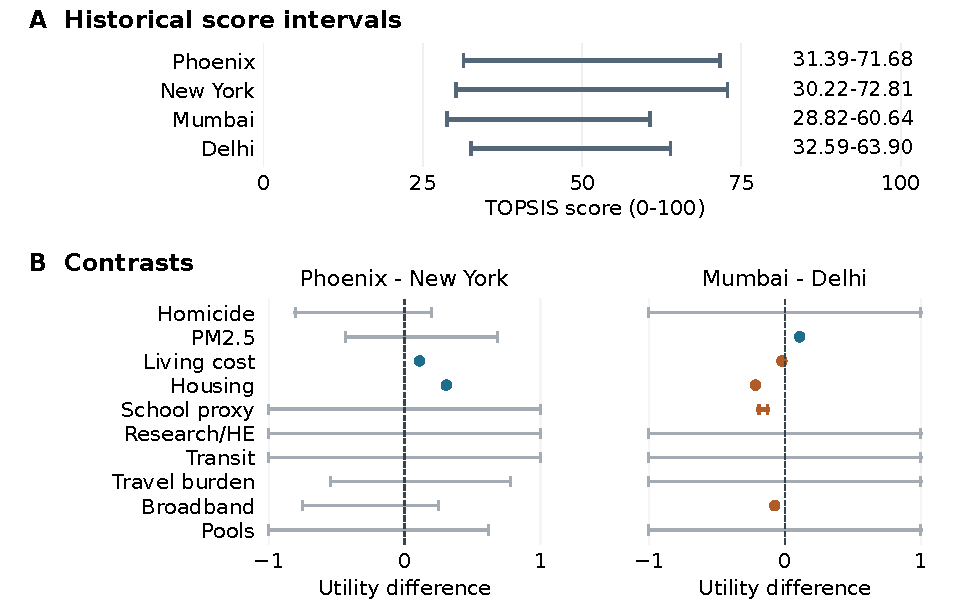
\includegraphics[width=\linewidth]{task4_v172_country_assets/country_contrasts.pdf}
\caption{Frozen auxiliary V117 country cases, separate from the primary sixteen cities.
Top: retained score intervals. Bottom: all twenty utility differences, first city minus second;
seven exclude zero. Positive differences favour the first city; negative differences favour
the second. Grey ranges leave direction unresolved. School resource retains
2024--25 school-location all-age XI--XII counts and nominal teacher-headcount allocation, not FTE.
Living cost and housing use 2025 Numbeo aggregates; air uses 2021 WHO monitoring means;
broadband uses the September 2026 index (July--September test window). Source years, boundaries and populations
differ. Ranges are conditional identification bounds, not confidence intervals;
neither pair identifies a necessary overall winner \cite{legacycase,numbeocase,whocase}.}
\label{fig:country-contrasts}
\end{figure}
